%`
%\nonstopmode
\hbadness=100000
\documentclass[a4paper, 12pt]{article}
\usepackage{amsmath,amsfonts,caption,float,geometry,graphicx,mathtools,pythonhighlight,textcomp,url,verbatim,subcaption,tabularx, longtable, ulem, hyperref, tikz} %,parskip
\geometry{ a4paper, total={170mm,257mm}, left=20mm, top=20mm}
\newcommand{\uul}[1]{\underline{\underline{#1}}}
\newcommand{\matr}[1]{\uul{\textbf{#1}}}
\newcommand{\apriori}[0]{\textit{a priori}}
\newcommand{\ve}[1]{\boldsymbol{#1}}
\newcommand{\flux}[0]{\ve{f}}
\newcommand{\xFW}[0]{x_{FW}}
\newcommand{\DFW}[0]{D_{FW}}
\newcommand{\LFW}[0]{L_{FW}}
\newcommand{\xBZ}[0]{x_{BZ}}
\newcommand{\DBZ}[0]{D_{BZ}}
\newcommand{\LBZ}[0]{L_{BZ}}
\newcommand{\eBZ}[0]{x_{BZ}+\delta}
\newcommand{\pythoncode}[2]{
\DeclareMathOperator*{\argmax}{arg\,max}
\DeclareMathOperator*{\argmin}{arg\,min}
\begin{adjustwidth}{-1.3cm}{-1.3cm}
\texttt{#1}
\inputpython{#2}{1}{1500}
\end{adjustwidth}
}
\usepackage[toc, page]{appendix}

\begin{document}
    
\begin{table}[!h]
\centering
\begin{tabular}{rl}
author:&Ocean Wong          \\
date:  &April 2025       \\
Organization:&Culham Centre for Fusion Energy
\end{tabular}
\end{table}
\hrule
\begin{abstract}
    To calculate crude approximations of the neutron flux(es) in the first wall and blanket of a fusion reactor in a reactor-design-agnostic manner, a semi-infinite model of the fusion neutron source, first-wall, and blanket are created. The one-group neutron transport equation is solved analytically while the multi-group neutron transport equation is solved numerically.
\end{abstract}
\emph{Keywords:} semi-infinite slab, fusion neutronics

\section{Simplification of the PROCESS model}
We would like to implement an elementary way of approximating the number of neutrons passing through and absorbed by the first wall and blanket of a fusion reactor in the reactor systems code PROCESS. Since most of PROCESS's plasma simulation models uses 1D model, with ``radial distance from the center of the plasma'' as the only coordinate, it is sensible to follow the same convention when performing our neutronics calculation, and assume that we are working with a cylindrical model (Figure~\ref{fig:radial_plot}).
\begin{figure}[H]
\centering
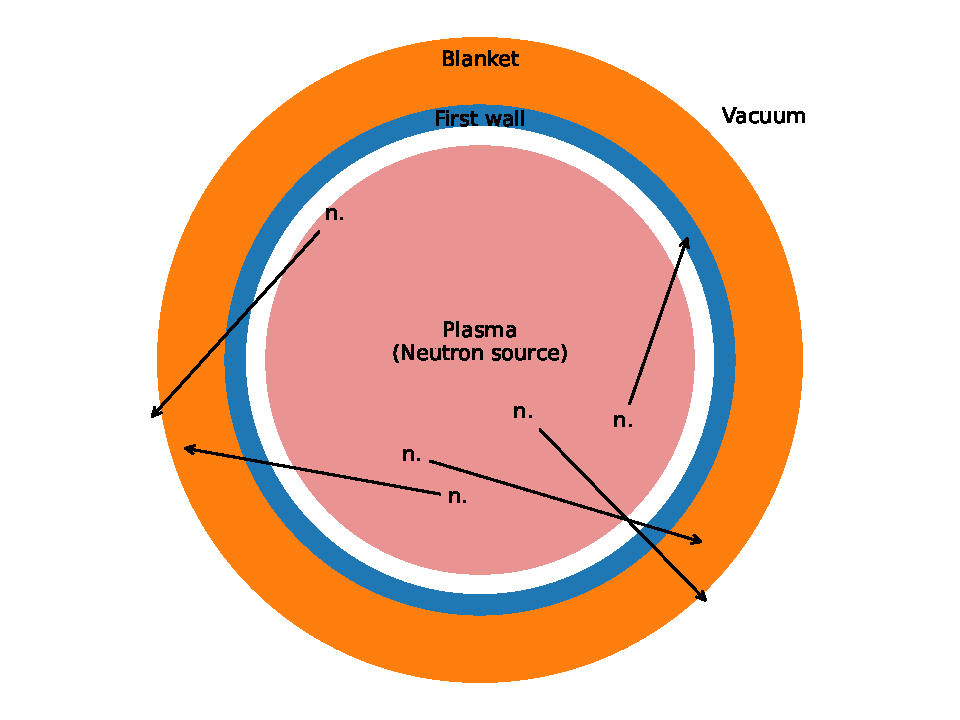
\includegraphics[width=0.5\textwidth]{radial_plot.pdf} %Stupid latex doesn't allow two dots in the filename.
\caption{The x-z cross-section of an example neutronics model appropriate for PROCESS.} \label{fig:radial_plot}
\end{figure}

Solving the neutron flux on this model using Equation~\ref{eq:TransportEqFicksLaw} would yield a sum involving Airy functions, which is a complex function not typically found in numerical solver packages.
Therefore, we choose to further simplify the geometry represented by Figure~\ref{fig:radial_plot}. By taking a horizontal slice of the figure at the plane of symmetry, we get:

\begin{figure}[H]
\centering
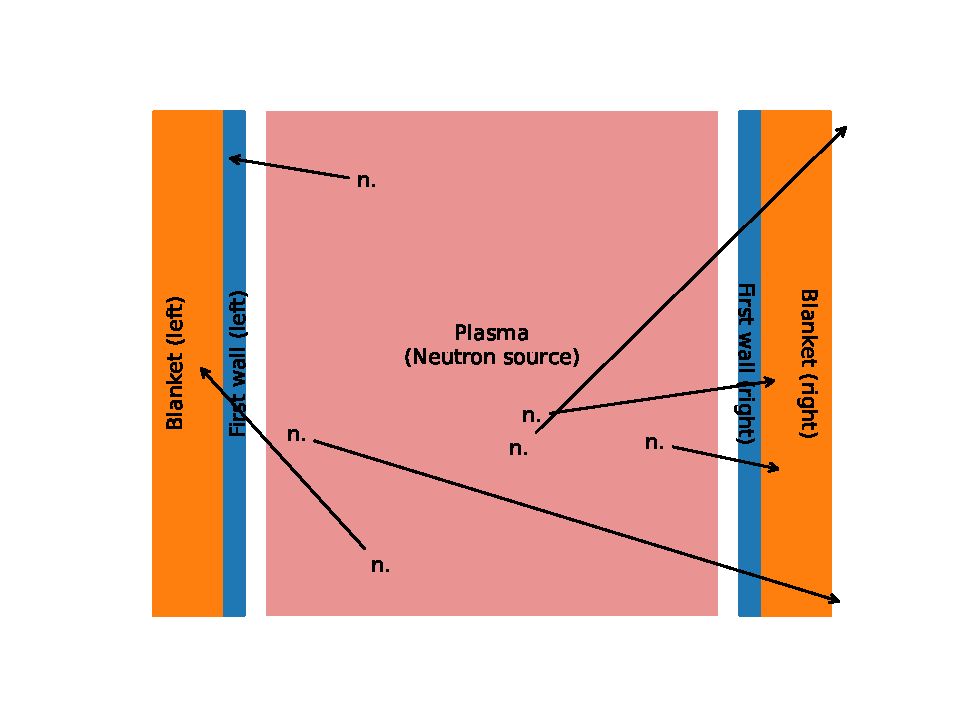
\includegraphics[width=0.5\textwidth]{semiinfinite_plot.pdf} %Stupid latex doesn't allow two dots in the filename.
\caption{A simple x cross-section of the an example neutronics model appropriate for PROCESS, obtained by taking a horiztonal slice of Figure~\ref{fig:radial_plot}.} \label{fig:semiinfinite_plot}
\end{figure}

Since the plasma only acts as a neutrons source, and is otherwise transparent to neutrons (i.e. neutrons passing through the plasma do not change direction), we can collapse the space between the left and right first wall, and approximate the plasma neutron source as a planar source instead (Figure~\ref{fig:collapsed_geometry}):

\begin{figure}[H]
\centering
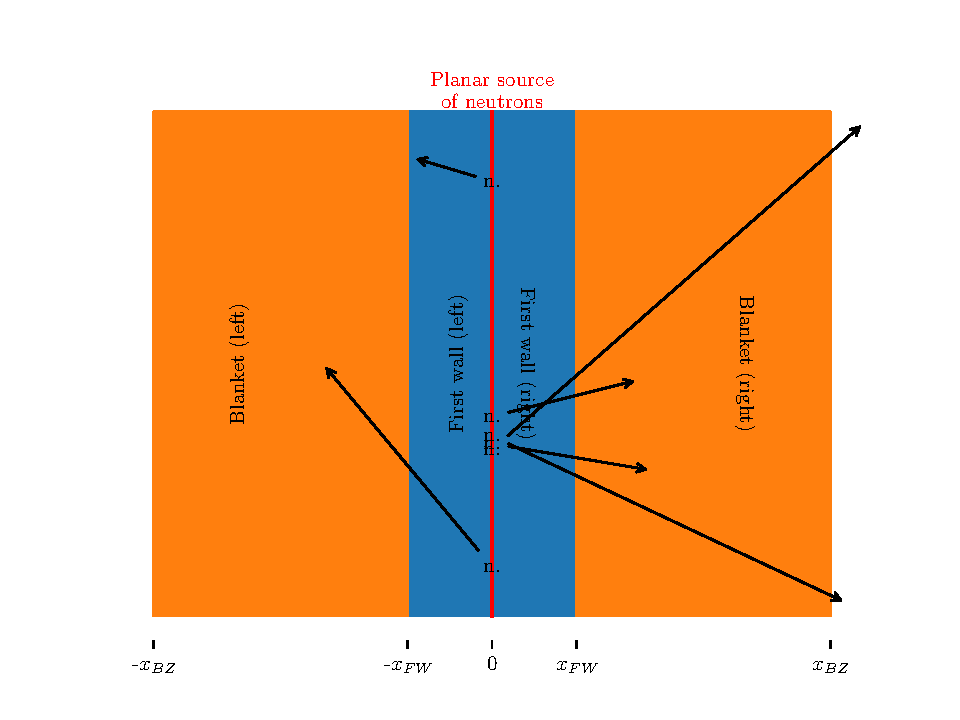
\includegraphics[width=0.5\textwidth]{collapsed_geometry.pdf} %Stupid latex doesn't allow two dots in the filename.
\caption{A simple x cross-section of the an example neutronics model appropriate for PROCESS, obtained by collapsing the neutron-transparent space in Figure~\ref{fig:semiinfinite_plot}. The blanket and first wall extends infinitely in the other two directions, i.e. vertically (up/down) and in/out of the page.} \label{fig:collapsed_geometry}
\end{figure}

Thus figure 3 represent a semi-infinite slab (finite thickness in the x-direction, but extends infinitely in the y- and z-directions).

The neutron transport equation is given by \cite{Duderstadt} in full as:
\begin{equation}\label{eq:FullTransportEq}
    \underbrace{\frac{1}{v}\frac{d\phi}{dt}}_{\text{time-dependence}} +
    \underbrace{\hat{\ve{\Omega}}\cdot\ve{\nabla}\phi}_{\text{streaming}} +
    \underbrace{\Sigma_t \phi}_{\text{collision/removal}} =
    \underbrace{\Sigma_s \phi}_{\text{scattering-in from other energy groups}} +
    \underbrace{\ve{S}}_{\text{other sources}}\,.
\end{equation}
All terms in Equation~\ref{eq:FullTransportEq} are implicitly dependent on angle ($\ve{\Omega}$), neutron energy, position ($\ve{r}$), and time.

\section{Simplification of the neutron transport equation}
Some of the variables are explained below:
\begin{itemize}
    \item $\Sigma_t = $ total macroscopic cross-section
    \item $\Sigma_s = $ (elastic) scattering macroscopic cross-section
    \item $\Sigma_i = $ macroscopic cross-section of reaction $i$ $= n_d \sigma_i = $ number density $\times$ microscopic cross-section of reaction $i$. Number density can be obtained by $N_d=\frac{N_A}{A}\rho=\frac{\text{Avogadro's number}}{\text{atomic number}}\times\text{density}$.
\end{itemize}

We also make the assumption that all neutron reactions that aren't elastically scattered are considered absorbed/lost due to transmutation, and that the fraction of atoms transmuted is insignificant for changing the neutronics properties of the material.

Duderstadt and Hamilton made several simplifications that makes Equation~\ref{eq:FullTransportEq} soluble.

\subsection{Removing time-dependence and fission sources}
The assumption of steady state operation and lack of fission sources in the media removes the leftmost and rightmost terms in Equation~\ref{eq:FullTransportEq}, giving:
\begin{equation}\label{eq:TransportEq3Terms}
    \hat{\ve{\Omega}}\cdot\ve{\nabla}\phi + \Sigma_t \phi =\Sigma_s \phi\,,
\end{equation}

$\phi$ is now only implicitly dependent on angle ($\ve{\Omega}$), neutron energy, and position ($\ve{r}$); but is time-invariant.

\subsection{Simplifying the streaming term}
Then, to turn the streaming term into something manageable, the neutron flux is assumed to be isotropic everywhere.
This is not entirely true in our case, where the neutron emitted from the plasma monoenergetic neutron source is assumed to be a narrow band of 14.1 MeV neutrons, such that neutrons streaming in the horizontal direction (perpendicular to the plane source in Figure~\ref{fig:collapsed_geometry}) will preferentially travel further, meaning that, far away from the neutron source, the distribution of neutron directions forms a spike pointed to the left/right, rather than a spherical cloud. However, this is deemed as an acceptable simplification required to proceed with the derivation.
This converts the ``neutron transport equation'' into a ``neutron diffusion equation'':
\begin{equation}\label{eq:TransportEqFicksLaw}
    -D\ve{\nabla}^2\phi + \Sigma_t \phi =\Sigma_s \phi\,.
\end{equation}

Note that the neutron flux profiles generated by solving Equation~\ref{eq:TransportEqFicksLaw} differs from the neutron flux profile generated by solving Equation~\ref{eq:FullTransportEq} near locations of abrupt changes, such as within several $\lambda_{tr}$ around the plane source or the vacuum boundary. However, this difference is only minute, as stated in p.159-160 of \cite{Duderstadt}.

The left most term is described as the Fick's Law term due to its visual similarity to the Fick's Law of Diffusion, despite its diffusion coefficient $D$ (defined in Section~\ref{sec:discretize}) having a different dimensionality (length) than when it appears in other fields of physics (area per unit time).

\subsection{Discretizing into energy groups}\label{sec:discretize}
The final step is to discretize the neutron spectrum into different energy groups, such that for each group's flux $\phi_i$, $\Sigma_t$ and $\Sigma_s$ are scalars, rather than functions requiring interpolation. (Note that $\phi_i$ is still implicitly dependent on position $\ve{r}$.) The larger the group number $i$, the higher the neutron lethargy, i.e. the less energy it has. (Remember that neutron lethargy is defined as $ln(\frac{E_0}{E})$, where $E_0$ is the initial energy of the neutron at its creation).

Assuming that neutrons can only downscatter (i.e. neutron energy $\gg$ thermal energy of the medium), we only have to sum up\footnote{Beware of confusion between summation sign $\sum$ and the macroscopic-cross-section sign $\Sigma$. It should be easy to tell them apart from context.} all of the scattered-in neutrons from higher energy neutrons.

\begin{equation}\label{eq:TransportEqFicksLawGroupwise}
    -D\ve{\nabla}^2\phi_i + \Sigma_t \phi_i =\sum_j^{j\le i} \Sigma_{s(i\rightarrow j)} \phi_j\,.
\end{equation}

The diffusion coefficient $D$ is given by p.136 of \cite{Duderstadt} as:
\begin{equation}
    D = \frac{1}{3\Sigma_{tr}} = \frac{\lambda_{tr}}{3} = \frac{1}{3(\Sigma_t - \frac{2}{3A}{\Sigma_s})}\,,
\end{equation}

where
\begin{itemize}
    \item $A$ is, as mentioned above, the atomic number of the medium being travelled through by the neutrons;
    \item $\lambda_{tr}$ is known as the mean-free-path of neutrons (for the given energy group and medium);
    \item $\Sigma_s$ is the sum of all scattering cross-sections from the current group $i$ down to all energy groups $j$ ($\Sigma_{s(i\rightarrow j)}$, where $j\ge i$, since upscatter is assumed impossible).
\end{itemize}

\subsection{Taking advantage of the symmetry in y- and z-direction}
Finally, we can remove the dependence on the other two spatial dimension, such that the diffusion equation can be simplified as:
\begin{align}
    -D \frac{d^2}{dx^2}\phi_i(x) + \Sigma_t \phi_i(x) &= \sum_j^{j\le i} \Sigma_{s(i\rightarrow j)} \phi_j(x)\\
    D \frac{d^2}{dx^2}\phi_i(x) &= \Sigma_t \phi_i(x)  -\sum_j^{j\le i} \Sigma_{s(i\rightarrow j)} \phi_j(x)\,.\label{eq:TransportEqX}
\end{align}

Now that the spatial dependence is more explicitly written ($\phi_i(x)$), we can begin solving for the solution.

\section{One-group solution}
This section's content is similar to the derivation on p.163-164, but the boundary conditions are different, hence a different result is produced.

If we assume the cross-sections for scattering and other reactions remains constant throughout the entire neutron spectrum, then we can re-use the same scalar values of $\Sigma_t$ and $\Sigma_s$ for all of the neutrons. Considering that we are evaluating the neutron flux emitted at $x=0$, propagating left and right into a purely-absorbing (i.e. non-fissile) medium (refer to Figure~\ref{fig:collapsed_geometry}), it is intuitive that the solution is some form of exponential decay on both sides of the source, where the neutron flux the further it travels into the first wall and blanket. And indeed, by applying the appropriate boundary conditions, we can obtain that result.

Let the incident neutron flux on the first wall be $\flux $ (SI unit: m$^{-2}$s$^{-1}$). Examining only the right-hand-side (i.e. $x>0$) of the model, we can derive the following:

\begin{equation}\label{eq:OneGroupDiffusionEqDifferentialForm}
    D \frac{d^2}{dx^2}\phi(x) = (\Sigma_t - \Sigma_s) \phi(x)\,,
\end{equation}
Solving this equation can be made easier if we first define a variable named $L$.
\begin{align}
    L^2 &=      \frac{D}{\Sigma_t-\Sigma_s}\nonumber\\
    L   &=\sqrt{\frac{D}{\Sigma_t-\Sigma_s}}\,.
\end{align}
For the one group case ($i = 1$ only), $\Sigma_s\equiv \Sigma_{s(1\rightarrow1)}$.
Note that the diffusion coefficient $D$ and macroscopic cross-sections $\Sigma_s$ and $\Sigma_t$ are going to be different in the first wall v.s. in the blanket, hence there are two different $D$, denoted $D_{FW}$ and $D_{BZ}$, and correspondingly, $L$ becomes $L_{FW}$ and $L_{BZ}$ respectively.

Let's express the thickness of the first wall and thickness of the blanket as ``first wall thickness'' = $x_{FW}$, ``blanket thickness'' = $x_{BZ} - x_{FW}$, such that the interface between the blanket and the vacuum boundary is located at $x_{BZ}$, as denoted in Figure~\ref{fig:collapsed_geometry}.

Solving Equation~\ref{eq:OneGroupDiffusionEqDifferentialForm} then gives the following two piecewise functions:
\begin{equation}\label{eq:OneGroupSwitchCase}
\phi(x) =
\begin{cases}
    c_1 e^{\frac{|x|}{L_{FW}}} + c_2 e^{-\frac{|x|}{L_{FW}}} & \text{ when }\quad\;     0<|x|\le x_{FW}\,,\\
    c_3 e^{\frac{|x|}{L_{BZ}}} + c_4 e^{-\frac{|x|}{L_{BZ}}} & \text{ when }x_{FW}<|x|\le x_{BZ} + \delta \,.
\end{cases}
\end{equation}
$c_1$, $c_2$, $c_3$, $c_4$ are all integration constants to be determined using the boundary conditions in Section~\ref{sec:OneGroupBoundaryCondition}.
An extrapolation length of $\delta = 0.7104\,\lambda_{tr} = 0.7104\times{3D_{BZ}}$ is added onto the vacuum boundary to obtain a more realistic flux profile, to counteract the inaccuracy introduced by approximating the transport equation with a diffusion equation.
The details of this deviation, and the why extending the vacuum boundary like such makes the diffusion approximation valid again, is explained in p.144 of \cite{Duderstadt}.

\subsection{Boundary conditions}\label{sec:OneGroupBoundaryCondition}
\begin{itemize}
    % \item Total number of reactions + Escaped neutrons $= \flux $.
    % \begin{itemize}
    %     \item Escaped flux $= \frac{\phi_i(x)}{2}$.
    %     \item Total number of (neutron-removing) reactions is the sum of all reactions excluding scattering reactions.
    %     \begin{align}
    %     \text{Total number of reactions per unit area} &= \int_{x>0}^{x=x_{FW}} \sum_i (\Sigma_{t,i} - \Sigma_{s,i}) \phi_i(x) dx\,,
    %     \intertext{in the one-group scenario, this is given by}
    %     \text{Total number of reactions per unit area} &= \int_{x>0}^{x=x_{FW}} (\Sigma_t - \Sigma_s) \phi(x) dx\,.
    %     \end{align}
    % \end{itemize}
    \item Neutron current density seeping out of either side of the plane source is equal to the incident neutron flux on the first wall, i.e.
    \begin{align}
        \ve{J}_x(0^+) &= \flux \nonumber\\
        -D \frac{d}{dx}\phi(x)\Bigg|_{x=0^+} &= \flux \,,\label{eq:b1}
    \end{align}
    for group 1 neutrons (i.e. neutrons in the same energy group as the source neutrons).
    \item Flux continuity at the first-wall-blanket interface $x_{FW}$, i.e.
    \begin{align}
        \phi(x_{FW} - \varepsilon) &= \phi((x_{FW} + \varepsilon))\label{eq:b2}
        \intertext{or more formally,}
        \lim_{\varepsilon\rightarrow0} (\phi(x_{FW} - \varepsilon)&-\phi((x_{FW} + \varepsilon))) = 0\,.\nonumber
    \end{align}
    \item Since the flux on either side of the first-wall-blanket interface is stable (i.e. time-invariant), the neutron current density from first wall to blanket = neutron current density from blanket to first wall at the interface $x_{FW}$, i.e.
    \begin{align}
        \ve{J}_x(x_{FW}-\varepsilon) &= \ve{J}_x(x_{FW}+\varepsilon)\nonumber\\
        -D_{FW} \frac{d}{dx}\phi(x)\Bigg|_{x_{FW}-\varepsilon} &= -D_{BZ} \frac{d}{dx}\phi(x)\Bigg|_{x_{FW}+\varepsilon}\nonumber\\
        D_{FW} \frac{d}{dx}\phi(x)\Bigg|_{x_{FW}-\varepsilon} &= D_{BZ} \frac{d}{dx}\phi(x)\Bigg|_{x_{FW}+\varepsilon}\,\label{eq:b3}
    \end{align}
    or more formally,
    \begin{equation}
        \lim_{\varepsilon\rightarrow0} \left( D_{FW} \frac{d}{dx}\phi(x)\Bigg|_{x_{FW}-\varepsilon} - D_{BZ} \frac{d}{dx}\phi(x)\Bigg|_{x_{FW}+\varepsilon} \right) = 0\nonumber
    \end{equation}
    \item The flux is expected to drop to zero at the \textit{extended boundary}, i.e.
    \begin{equation}
        \phi(x_{BZ} + \delta) = 0\label{eq:b4}
    \end{equation}
\end{itemize}

After a somewhat-intensive evaluation of simultaneous Equations~\ref{eq:b1}, \ref{eq:b2}, \ref{eq:b3}, and \ref{eq:b4}, we have:

\begin{align}
    c_2 &= \left(\frac{ \flux }{2}\right) &\cdot e^{\frac{\xFW }{\LFW } } &\frac{ \frac{\LFW }{\DFW } + \frac{\LBZ }{\DBZ }\tanh\left(\frac{\eBZ -\xFW}{\LBZ } \right)}{\cosh\left(\frac{\xFW }{\LFW }\right) + \sinh{\left(\frac{\xFW }{\LFW }\right)} \tanh\left(\frac{\eBZ -\xFW}{\LBZ } \right) \frac{\DFW }{\LFW }\frac{\LBZ }{\DBZ }}\label{eq:b1a}\\
    c_1 &= c_2 - \frac{\LFW }{\DFW }\flux \nonumber\\
    c_4 &= \left(\frac{\flux }{2}\frac{\LFW }{\DFW } e^{\frac{\xFW }{\LFW } }\right) &\cdot e^{\frac{\eBZ }{\LBZ }} &\frac{1-\tanh\left(\frac{\xFW }{\LFW }\right)}{\frac{\DBZ }{\LBZ } \frac{\LFW }{\DFW } \cosh\left(\frac{\eBZ-\xFW}{\LBZ }\right) + \tanh\left(\frac{\xFW }{\LFW }\right) \sinh\left(\frac{\eBZ - \xFW }{\LBZ }\right)} \\
    c_3 &= -c_4 e^{-\frac{2(\eBZ )}{\LBZ }}\nonumber\\
        &= \left(-\frac{\flux }{2} \frac{\LFW }{\DFW } e^{\frac{\xFW }{\LFW } }\right) &\cdot e^{-\frac{\eBZ }{\LBZ }} &\frac{1-\tanh\left(\frac{\xFW }{\LFW }\right)}{\frac{\DBZ }{\LBZ } \frac{\LFW }{\DFW } \cosh\left(\frac{\eBZ-\xFW}{\LBZ }\right) + \tanh\left(\frac{\xFW }{\LFW }\right) \sinh\left(\frac{\eBZ - \xFW }{\LBZ }\right)}\label{eq:b4a}
\end{align}

Finally, this yields a flux profile as shown in Figure~\ref{fig:OneGroupFlux}.
\begin{figure}
  \begin{subfigure}[b]{0.4\textwidth}
    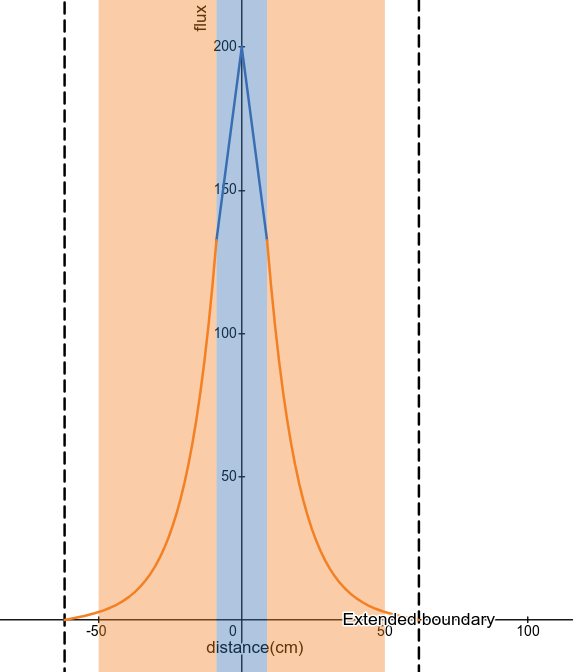
\includegraphics[width=\textwidth]{OneGroupFluxBlanketAbs.png}
    \caption{The case where the total macroscopic cross-section of the blanket is greater than that of the first wall.}
    \label{fig:OneGroupFluxBlanketAbs}
  \end{subfigure}
  \hfill
  \begin{subfigure}[b]{0.4\textwidth}
    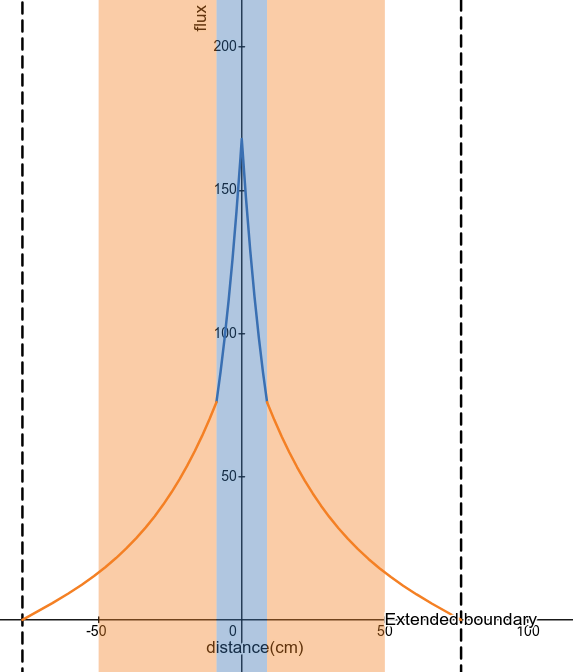
\includegraphics[width=\textwidth]{OneGroupFluxFWAbs.png}
    \caption{The case where the total macroscopic cross-section of the first wall is greater than that of the blanket.}
    \label{fig:OneGroupFluxFWAbs}
  \end{subfigure}
  \caption{Examples of the neutron flux profiles predicted by the neutron diffusion equation using the one-group model under a variety of combination of cross-section ratios.}\label{fig:OneGroupFlux}
\end{figure}

Combining Equation~\ref{eq:OneGroupSwitchCase} and the constants in Equations~\ref{eq:b1a} to \ref{eq:b4a}, the neutron flux at any depth $|x|<\xBZ, x\neq 0$ can be predicted.

\subsection{Rates}
The average number of neutron-induced reactions per unit volume between the depths $x=a$ to $x=b$,
\begin{equation}
    \text{reaction rate} = \int_{x=a}^{x=b}\Sigma\phi(x)dx\,,
\end{equation}
The indefinite integral is 
\begin{equation}
\LFW (c_1 e^{\frac{|x|}{L_{FW}}} - c_2 e^{-\frac{|x|}{L_{FW}}})+C
\end{equation}
 for the first wall region and 
\begin{equation}
\LBZ (c_3 e^{\frac{|x|}{L_{BZ}}} - c_4 e^{-\frac{|x|}{L_{BZ}}})+C
\end{equation}
  in the blanket region.

We can replace $\Sigma$ with $(\Sigma_t-\Sigma_s)$ to count only non-scattering reactions, or we can replace it with $\Sigma_t$ to count all reactions.

For any interface located at position $x'$, we can also calculate the number of neutrons passing through every unit area of this interface using the equation:
\begin{equation}
    \text{Neutron escape rate} = -D \frac{d}{dx}\phi(x)\Bigg|_{x'}\label{eq:EscapedFlux}
\end{equation}
\begin{equation}\label{eq:ExitFW}
    \text{rate of neutrons exiting the first wall} = -\frac{\DFW }{\LFW }\left(c_1 e^{\frac{\xFW }{\LFW }} - c_2e^{-\frac{\xFW }{\LFW }}\right)\,,
\end{equation}
\begin{equation}\label{eq:EnterBlanket}
    \text{rate of neutrons entering the blanket} = -\frac{\DBZ }{\LBZ}\left(c_3 e^{\frac{\xFW }{\LBZ }} - c_4 e^{-\frac{\xFW }{\LBZ }}\right)\,.
\end{equation}
The quantity in Equation~\ref{eq:ExitFW} and \ref{eq:EnterBlanket} should be the same by construction, as enforced by condition~\ref{eq:b3}. Evaluating the latter expression, the net number of neutrons streaming from left to right across the first-wall-blanket interface per unit area
\begin{align}
    =& c_4 \frac{\DBZ }{\LBZ }e^{-\frac{(\eBZ )}{\LBZ }} 2\cosh\left(\frac{\eBZ -\xFW}{\LBZ } \right)\nonumber\\
    % =& \frac{\flux\frac{\LFW }{\DFW }\frac{\DBZ }{\LBZ } e^{\frac{\xFW }{\LFW } } \cosh\left(\frac{\eBZ -\xFW}{\LBZ } \right) \left(1-\tanh\left(\frac{\xFW }{\LFW }\right)\right)}{\frac{\DBZ }{\LBZ } \frac{\LFW }{\DFW } \cosh\left(\frac{\eBZ-\xFW}{\LBZ }\right) + \tanh\left(\frac{\xFW }{\LFW }\right) \sinh\left(\frac{\eBZ - \xFW }{\LBZ }\right)}
    =& \frac{\flux e^{\frac{\xFW }{\LFW } } \left(1-\tanh\left(\frac{\xFW }{\LFW }\right)\right)}{1 + \tanh\left(\frac{\xFW }{\LFW }\right) \tanh\left(\frac{\eBZ - \xFW }{\LBZ }\right) \frac{\DFW }{\LFW }\frac{\LBZ }{\DBZ }}\,.
\end{align}
As for the number of neutrons escaping the model into the vacuum (void), 
\begin{align}
    &\text{rate of neutrons exiting the blanket (lost to the void)} = -\frac{\DBZ }{\LBZ}\left(c_3 e^{\frac{\xBZ }{\LBZ }} - c_4 e^{-\frac{\xBZ }{\LBZ }}\right)\nonumber\\
    =& c_4 \frac{\DBZ }{\LBZ } e^{-\frac{\eBZ }{\LBZ }} 2\cosh\left(\frac{\delta}{\LBZ }\right)\nonumber\\
    =& \left(\flux\frac{\LFW }{\DFW }\frac{\DBZ }{\LBZ } e^{\frac{\xFW }{\LFW } }\right) \frac{\cosh\left(\frac{\delta}{\LBZ }\right)\left(1-\tanh\left(\frac{\xFW }{\LFW }\right)\right)}{\frac{\DBZ }{\LBZ } \frac{\LFW }{\DFW } \cosh\left(\frac{\eBZ-\xFW}{\LBZ }\right) + \tanh\left(\frac{\xFW }{\LFW }\right) \sinh\left(\frac{\eBZ - \xFW }{\LBZ }\right)}
\end{align}

\section{Multi-group solution}
To extend this model to account for reaction cross-section variation as neutron lethargy increases, one can replace the neutron spectrum $\phi(x)$ with a position-dependent vector $\ve{\phi}(x)$. Analysing $\phi_1(x)$ would give the same result as Equation~\ref{eq:OneGroupSwitchCase}. Meanwhile, solving forhigher lethargy neutron groups, we have:
\begin{align}
    D \frac{d^2}{dx^2}\phi_2(x) &= \Sigma_t \phi_2(x)  - \Sigma_{s(1\rightarrow 2)} \phi_1(x)\label{eq:phi2}\\
    D \frac{d^2}{dx^2}\phi_3(x) &= \Sigma_t \phi_3(x)  - \Sigma_{s(1\rightarrow 3)} \phi_1(x) - \Sigma_{s(2\rightarrow 3)} \phi_2(x)\label{eq:phi3}\\
    D \frac{d^2}{dx^2}\phi_4(x) &= \Sigma_t \phi_4(x)  - \Sigma_{s(1\rightarrow 4)} \phi_1(x) - \Sigma_{s(2\rightarrow 4)} \phi_2(x) - \Sigma_{s(3\rightarrow 4)} \phi_3(x)\label{eq:phi4}\\
    &\vdots \nonumber
\end{align}
Since the closed-form expression for $\phi_1$, we deduce the closed-form expression for $\phi_2$ with Equation~\ref{eq:phi2}; and therefore we can deduce the closed-form expression for $\phi_3$ with Equation~\ref{eq:}

Here, we assume the emitted neutrons are monoenergetic, produced at 14.06MeV.

Since no other groups can scatter neutrons into it, group 1's neutron flux is going to be of the same form that given by Equation~\ref{eq:OneGroupSwitchCase}. The only difference is that the constants $D$, $L$, $\delta$ in Equations~\ref{eq:b1}, \ref{eq:b2}, \ref{eq:b3}, and \ref{eq:b4} are swapped in for group 1's group-wise constants instead of the one-group constants used in Section~\ref{sec:OneGroupBoundaryCondition}.

\bibliographystyle{unsrt}
\bibliography{NeutronDiffusion}
\end{document}
